\documentclass{article}
\usepackage{../../../../format}
\usepackage{hyperref}
\definecolor{links}{HTML}{2A1B81}
\hypersetup{colorlinks,linkcolor=,urlcolor=blue}
\usetikzlibrary{shapes.misc}
\usetikzlibrary{shapes.geometric, arrows, positioning}
\usepackage{minted}



\begin{document}

\begin{center}
	\underline{\huge Dynamic memory management}
\end{center}






\section{Arrays in C}
\begin{minted}{c}
int a[10];
\end{minted}

\begin{itemize}
\item declares a fixed size array holding ten \verb!int! values

\begin{center}
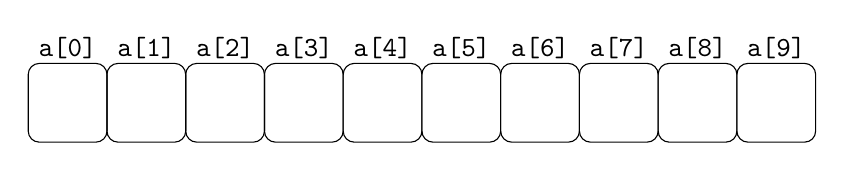
\begin{tikzpicture}
\begin{scope}[shift={(9,0)}]
\draw[rounded corners] (0, 0) rectangle (1, 1) {};
\node at (0.5,1.2) {\texttt{a[9]}};
\end{scope}
\begin{scope}[shift={(8,0)}]
\draw[rounded corners] (0, 0) rectangle (1, 1) {};
\node at (0.5,1.2) {\texttt{a[8]}};
\end{scope}
\begin{scope}[shift={(7,0)}]
\draw[rounded corners] (0, 0) rectangle (1, 1) {};
\node at (0.5,1.2) {\texttt{a[7]}};
\end{scope}
\begin{scope}[shift={(6,0)}]
\draw[rounded corners] (0, 0) rectangle (1, 1) {};
\node at (0.5,1.2) {\texttt{a[6]}};
\end{scope}
\begin{scope}[shift={(5,0)}]
\draw[rounded corners] (0, 0) rectangle (1, 1) {};
\node at (0.5,1.2) {\texttt{a[5]}};
\end{scope}
\begin{scope}[shift={(4,0)}]
\draw[rounded corners] (0, 0) rectangle (1, 1) {};
\node at (0.5,1.2) {\texttt{a[4]}};
\end{scope}
\begin{scope}[shift={(3,0)}]
\draw[rounded corners] (0, 0) rectangle (1, 1) {};
\node at (0.5,1.2) {\texttt{a[3]}};
\end{scope}
\begin{scope}[shift={(2,0)}]
\draw[rounded corners] (0, 0) rectangle (1, 1) {};
\node at (0.5,1.2) {\texttt{a[2]}};
\end{scope}
\begin{scope}[shift={(1,0)}]
\draw[rounded corners] (0, 0) rectangle (1, 1) {};
\node at (0.5,1.2) {\texttt{a[1]}};
\end{scope}
\draw[rounded corners] (0, 0) rectangle (1, 1) {};
\node at (0.5,1.2) {\texttt{a[0]}};
\end{tikzpicture}
\end{center}

\item \verb!a[i]! is the \verb!i!th element of the array
\item \verb!sizeof(a) = 10 * sizeof(int) = 40! bytes
\item The array is stored in memory as a single contiguous block that is 40 bytes (10 \verb!int!s) in size

\item Note that \verb!sizeof(a) / sizeof(a[0])=10!
\begin{itemize}
\item This is a common way of checking the number of elements in an array.
\item We can't pass an array to a function, but we can pass a pointer to it. The line above will not work correctly on a pointer, so we will need to pass the length of the array too.
\end{itemize}
\end{itemize}



\section{Strings}
\begin{itemize}
\item Are represented as an array of characters
\begin{minted}{c}
char a[] = "Hello worlds";
char b[13];
b = a; // Not allowed
char *c;
c = a;
\end{minted}
\item will set pointer \verb!c! to same address as \verb!a!
\item assignment of an array to array is not supported in C
\item unlike \verb!struct! as we saw last lecture
\item \verb!strcpy(b,a);!  first argument is the destination, ordered like assignment above
\begin{itemize}
\item need to \verb!#include<string.h>!
\end{itemize}
\end{itemize}
\begin{minted}{c}
char a[] = "Hello";
strlen(a) = 5;
sizeof(a) = 6;
\end{minted}

\begin{itemize}
\item Strings are null terminated -- important when allocating space to store them
\begin{minted}{c}
printf("%s %c\n", a, a[0]);
\end{minted}
\item Output is:
\begin{minted}{c}
Hello H
\end{minted}

\item If you use the variable \verb!a! on its own, it represents the memory address of the start of the string
\end{itemize}



\section{Pointers, strings and arrays}

\begin{center}
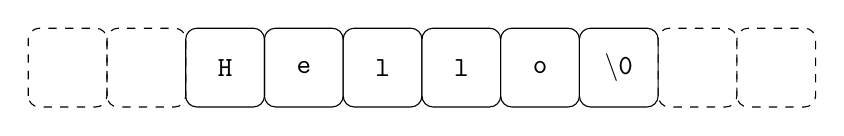
\begin{tikzpicture}
\begin{scope}[shift={(7,0)}]
\draw[rounded corners,dashed] (0, 0) rectangle (1, 1) {};
\end{scope}
\begin{scope}[shift={(6,0)}]
\draw[rounded corners,dashed] (0, 0) rectangle (1, 1) {};
\end{scope}
\begin{scope}[shift={(5,0)}]
\draw[rounded corners] (0, 0) rectangle (1, 1) {};
\node at (0.5,0.5) {\texttt{\textbackslash0}};
\end{scope}
\begin{scope}[shift={(4,0)}]
\draw[rounded corners] (0, 0) rectangle (1, 1) {};
\node at (0.5,0.5) {\texttt{o}};
\end{scope}
\begin{scope}[shift={(3,0)}]
\draw[rounded corners] (0, 0) rectangle (1, 1) {};
\node at (0.5,0.5) {\texttt{l}};
\end{scope}
\begin{scope}[shift={(2,0)}]
\draw[rounded corners] (0, 0) rectangle (1, 1) {};
\node at (0.5,0.5) {\texttt{l}};
\end{scope}
\begin{scope}[shift={(1,0)}]
\draw[rounded corners] (0, 0) rectangle (1, 1) {};
\node at (0.5,0.5) {\texttt{e}};
\end{scope}
\draw[rounded corners] (0, 0) rectangle (1, 1) {};
\node at (0.5,0.5) {\texttt{H}};
\begin{scope}[shift={(-1,0)}]
\draw[rounded corners,dashed] (0, 0) rectangle (1, 1) {};
\end{scope}
\begin{scope}[shift={(-2,0)}]
\draw[rounded corners,dashed] (0, 0) rectangle (1, 1) {};
\end{scope}
\end{tikzpicture}
\end{center}

\begin{minted}{c}
char a[] = "Hello";
char *a = "Hello";
\end{minted}

\begin{itemize}
\item These are equivalent declarations, and create the identical bytes in memory, as shown above.
\item \emph{Warning:} using \verb!sizeof(a)! will give \verb!6! in the first case (the size of the array) and \verb!8! in the second case (the size of the pointer).\
\item In the second case, the string \verb!"Hello"! is constant and cannot be modified.
\item Pointers and arrays are often used interchangeably
\end{itemize}



\section{Pointer arithmetic}
\begin{itemize}
\item Pointer arithmetic accounts for the base type of the items: 

\begin{minted}{c}
int a[10];
int *pa;

pa = &a[0];
pa = a;
\end{minted}

\begin{center}
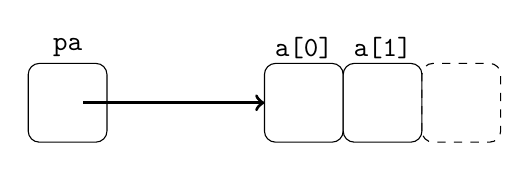
\begin{tikzpicture}
\draw[rounded corners] (0, 0) rectangle (1, 1) {};
\draw[rounded corners] (1, 0) rectangle (2, 1) {};
\draw[rounded corners,dashed] (2, 0) rectangle (3, 1) {};
\node at (0.5,1.2) {\texttt{a[0]}};
\node at (1.5,1.2) {\texttt{a[1]}};

\draw[rounded corners] (-3, 0) rectangle (-2, 1) {};
\draw[very thick,->] (-2.3,0.5) -- (0,0.5);
\node at (-2.5,1.2) {\texttt{pa}};
\end{tikzpicture}
\end{center}

\begin{minted}{c}
pa = &a[1];
pa = (a+1);
\end{minted}

\begin{center}
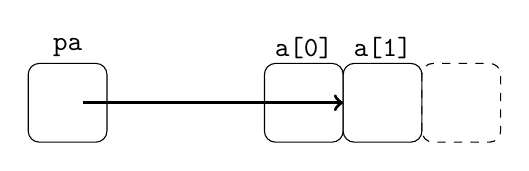
\begin{tikzpicture}
\draw[rounded corners] (0, 0) rectangle (1, 1) {};
\draw[rounded corners] (1, 0) rectangle (2, 1) {};
\draw[rounded corners,dashed] (2, 0) rectangle (3, 1) {};
\node at (0.5,1.2) {\texttt{a[0]}};
\node at (1.5,1.2) {\texttt{a[1]}};

\draw[rounded corners] (-3, 0) rectangle (-2, 1) {};
\draw[very thick,->] (-2.3,0.5) -- (1,0.5);
\node at (-2.5,1.2) {\texttt{pa}};
\end{tikzpicture}
\end{center}

\item The two pairs of statements above are equivalent using array or pointer notation: \verb!+1! translates to \verb!+4! bytes (1 \verb!int!)
\end{itemize}



\section{Pointer oddities}
\begin{itemize}
\item In C if I write \verb!a[x]! this works by adding \verb!x! to \verb!a! to find the pointer
\item Hence \verb!a[x]! is the same as \verb!*(a+x)!
\item This seems fine if I write \verb!a[2]!
\item But what if I write \verb!2[a]!?
\item It compiles and works!
\item See \verb!array.c!
\end{itemize}
\inputminted{c}{array.c}
All of these are valid

\subsection{More oddities}
\begin{itemize}
\item \verb!a[-4]! ?
\item Interpreted as \verb!*(a + -4)!

\item Is the following valid?
\begin{minted}{c}
int *p;
int i = 5;
int j = 20;
p = &i;
printf("%d %d\n", p[0], p[1]);
\end{minted}

\item \mintinline{c}{p[0]} will be 5
\item \mintinline{c}{p[1]} could be anything, it's just the next memory location
\end{itemize}



\section{Peeking at memory}
\begin{itemize}
\item Can look at bits of memory
\item See \verb!peek.c!
\item Can find adjacent local variables and parameters
\item Easy to make mistakes
\item Cannot tell what data is by looking at it
\end{itemize}



\section{Breaking things}
\begin{itemize}
\item We can use random numbers to write random values in random places
\item See \verb!break.c!
\item This can upset the system
\item Segmentation fault occurs: hardware tells OS a memory access is not allowed
\item Sometimes it goes on for a shockingly long time
\item Sometimes the last number is very strange: why?
\end{itemize}

\section{Pointer safety}
\begin{itemize}
\item Pointers can cause hard to diagnose errors in programs

\item For example functions returning pointers to local variables can cause difficult to catch errors when the memory is released back to the runtime system and reused at some time later in the program

\item Always set pointers to \verb!NULL! when they are no longer required

\item Always use a simple guard before using pointers e.g.:
\verb~assert(ptr != NULL);~ from \verb!<assert.h>!

\item There are various tools e.g. Valgrind that can detect many such errors at runtime (at the cost of massive slowdown and greatly increased memory-usage)
\end{itemize}



\section{Dynamic memory allocation}


\begin{itemize}
\item Variables and arrays provide fixed size allocation
\item What if the memory needed cannot be pre-determined?
\item There is a need to be able to dynamically request variable sized blocks of memory from the runtime system
\item Close integration between C and Unix (and other OS's)
\item Requesting memory at run-time
\end{itemize}



\begin{minipage}{0.4\textwidth}


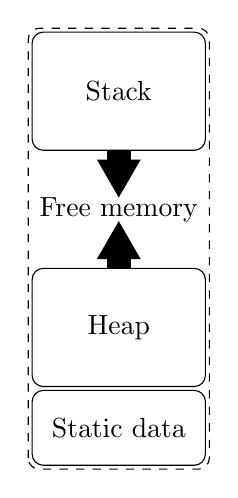
\begin{tikzpicture}
\tikzset{
  myarrow/.style = {line width=1mm, draw=black, -triangle 60, fill=white,postaction={draw, line width=3mm, shorten >=3mm, -}}
}

\draw[rounded corners] (-2.1, 0.5) rectangle (0.1, 1.45) {};
\node at (-1,0.975) {Static data};
\draw[rounded corners] (-2.1, 1.5) rectangle (0.1, 3) {};
\node at (-1,2.25) {Heap};
\draw[rounded corners] (-2.1, 4.5) rectangle (0.1, 6) {};
\node at (-1,5.25) {Stack};
\node at (-1,3.75) {Free memory};

\draw[rounded corners,dashed] (-2.15, 0.45) rectangle (0.15, 6.05) {};

\draw [myarrow] (-1,3) -- (-1,3.6);
\draw [myarrow] (-1,4.5) -- (-1,3.9);

\end{tikzpicture}


\end{minipage}




\section{Memory Layout}
\begin{itemize}
\item Stack
\begin{itemize}
\item Stores ``temporary'' data
\item Variables in a function
\item Function header
\item Small data
\end{itemize}
\item Heap
\begin{itemize}
\item Used for storing more long-term data
\item YOU control what is in the Heap and when it is released
\item Much more space than the Stack
\end{itemize}
\item Static Data
\begin{itemize}
\item Data that stays in memory for the duration of the program
\end{itemize}
\end{itemize}





\section{Memory Allocation: \texttt{malloc() <stdlib.h>}}
\begin{itemize}
\item Function prototype for \verb!malloc()!
\begin{minted}{c}
void *malloc(size_t  size);
\end{minted}
\item Allocates a contiguous block of memory \verb!size! bytes long
\item The return type is \verb!void*!, which is a generic pointer type that can be used with all types
\item \verb!malloc()! returns a \verb!NULL! pointer if it fails to allocate the requested memory
\item \textbf{Always test for \texttt{NULL} return!}
\begin{itemize}
\item An aside: By default, Linux follows an optimistic memory allocation strategy: if \verb!malloc()! returns a non-\verb!NULL! value, this is no guarantee that the memory is really available.
The operating system actually allocates the memory when you try to use it for the first time; if the system runs out of memory, a process will be killed by the Out Of Memory (OOM) killer.
\end{itemize}
\end{itemize}



\subsection{\texttt{malloc()} example of use}
\begin{minted}{c}
#define SIZE 41 * sizeof(char)

char *line; 
line = malloc(SIZE);
if ( line == NULL ) {
  printf( "Error in malloc() \n" );
  exit(1);
}
\end{minted}

\begin{itemize}
\item N.B. The return value of \verb!malloc()! is automatically cast from \verb!void*! to \verb!char*!
\begin{itemize}
\item Pointers pointing to any object are automatically converted to \verb!void*! pointers and vice versa as required.
\item Conversions between other sorts of pointers with different types may cause problems due to alignment issues.
\end{itemize}
\end{itemize}



\section{Memory de-allocation: \texttt{free() <stdlib.h>}}
\begin{minted}{c}
void free(void *ptr);
\end{minted}

\begin{itemize}
\item Takes a generic pointer to a block of memory and returns the memory for reuse by \verb!malloc()!

\item If you ``forget'' about memory you have \verb!malloc()!ed and don't \verb!free()! it then you have a ``memory leak''

\item ``Memory leaks'' can be very dangerous and difficult to trace, see also garbage collection in Java/Python
\item Can eventually use up all memory

\item \verb!free()! has no return value, so even if you pass it a pointer not allocated by \verb!malloc()!, it will process it!
\end{itemize}



\subsection{\texttt{free()} example of use}
\begin{minted}{c}
// allocate some memory
line = malloc(SIZE);

// use line in the program 

free( line ); // return memory to the O/S
line = NULL;  // set pointer to NULL
\end{minted}

\begin{itemize}
\item Errors from continuing to use a pointer after the memory has been released can be very hard to detect

\item N.B. line is implicitly cast to a \verb!void*! pointer
\end{itemize}



\section{Memory allocation: \texttt{calloc() <stdlib.h>}}
\begin{itemize}
\item Function prototype for \verb!calloc()!
\begin{minted}{c}
void *calloc( size_t n, size_t  size );
\end{minted}
\item Allocates a contiguous block of memory of \verb!n! elements each of \verb!size! bytes long, initialised to all bits \verb!0!

\item Useful to ensure old data is not reused inappropriately

\item The return type is \verb!void*!, which is a generic pointer type that can be used for all types

\item \verb!calloc()! returns a \verb!NULL! pointer if it fails to allocate the requested memory
\item Always test for \verb!NULL! return!
\end{itemize}



\section{Memory allocation: \texttt{realloc() <stdlib.h>}}
\begin{itemize}
\item Function prototype for \verb!realloc()!
\begin{minted}{c}
void *realloc( void *ptr, size_t  size );
\end{minted}

\item Allows a dynamic change in size of an allocated block of memory pointed to by \verb!ptr!
\begin{itemize}
\item \verb!ptr! must point to memory previously allocated by \verb!malloc()!, \verb!calloc()! or \verb!realloc()!
\end{itemize}

\item Will move and copy contents if it needs to, freeing original block
\item \verb!realloc()! returns a \verb!NULL! pointer if it fails. \textbf{Check for this}!
\item Cf. ArrayList in Java
\end{itemize}



\subsection{\texttt{realloc()} example}
\begin{itemize}
\item Simple program that takes integers typed in by the user and stores them in an array

\item Each time the array becomes full, it is dynamically increased in size to hold more numbers

\item Contains a key function \verb!getline2()!, which reads the integers from the command line
\end{itemize}



%\section{}
\begin{minted}{c}
int getline2(char line[], int max) {
    int nch = 0;
    int c;
    max = max - 1;/* leave room for '\0' */
    while((c = getchar()) != 'q') {
        if(c == '\n')
            break;
        if(nch < max) {
            line[nch] = c;
            nch = nch + 1;
        }
    }
    if(c == 'q' && nch == 0)
        return 'q';
    
    line[nch] = '\0';
    return nch;
}
\end{minted}


\begin{itemize}
\item \verb!getline2()!

\item Uses \verb!getchar()! to read in characters as they are typed

\item Runs in a loop until a \verb!'q'! or a newline is encountered

\item Reads in the characters typed by the user one by one and stores them in the array line

\item When the character \verb!'\n'! is pressed, the function returns, via use of the \verb!break! statement to exit a loop

\item No checking performed to see if the input is an integer
\end{itemize}



%\section{}
\begin{minted}{c}
ip = malloc(array_size * sizeof(int));
while( getline2(line, MAXLINE) != 'q' ) {
    if(nitems >= array_size ) {/* increase allocation */
        int *newp;
        array_size += INCREASE ;
        newp = realloc(ip, array_size * sizeof(int));
        printf("<< Expanding by %d to size %d >>\n",
                            INCREASE, array_size );
        if(newp == NULL) {
            printf("out of memory\n");
            exit(1);
        }
        ip = newp;
    }
    ip[nitems++] = atoi(line);
}
\end{minted}

\begin{itemize}
\item \verb!main()!

\item Uses \verb!getline2()! to read in a line of text

\item Creates an array to store current line of text,  \verb!line!

\item Creates a second array to store the integers entered: \verb!ip!

\item As soon as \verb!ip! is full, \verb!realloc()! is called to resize the array
\end{itemize}



\section{\texttt{atoi() <stdlib.h>}}
\begin{minted}{c}
int atoi(const char *s);
\end{minted}

\begin{itemize}
\item Converts a string pointed to by  s  to an integer

\item Also see \verb!atof()!, \verb!atol()! and \verb!atoll()! (since C99) equivalents

\item To convert from an integer to a string use :

\begin{minted}{c}
int sprintf( char *s, char *format, <value list> );
\end{minted}

\item Where the value list is the variables used in the format string
\end{itemize}

\end{document}
